\begin{wrapfigure}[17]{R}[0pt]{0.5\textwidth}
  % R - floating; r - h! [narrow lines] <- reduce whitespace below
  \centering
  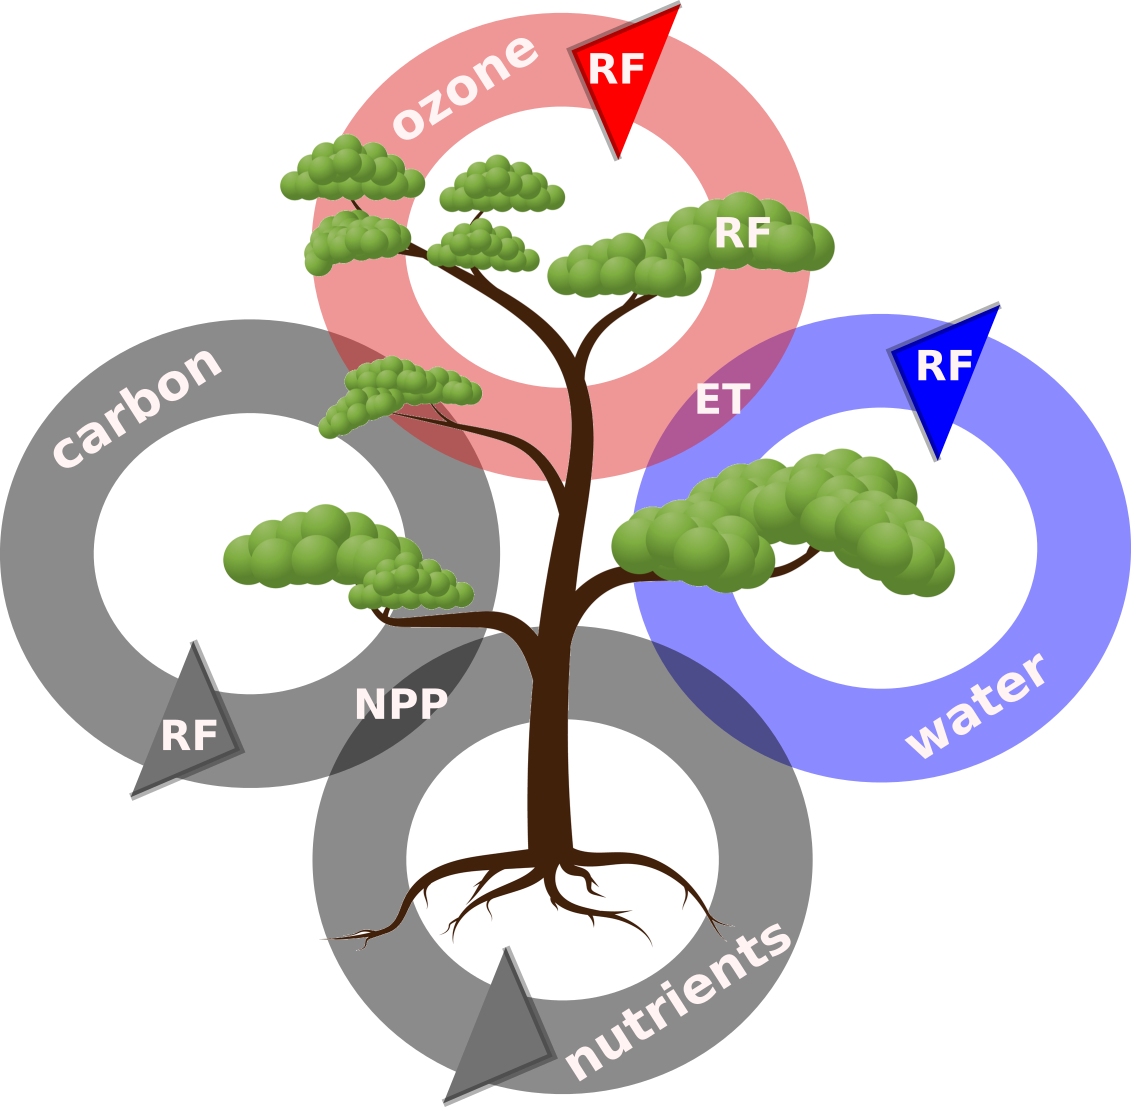
\includegraphics[width=0.48\textwidth]{ozone_es_scheme}
  \caption{Schematic view of the importance of ozone in \glspl{esm}. Ozone inflicts damage to vegetation. Ozone affects photosynthesis negatively and hence \gls{npp} ($\rightarrow$ carbon cycle). Ozone affects opening and closing of stomata (positively and negatively) and hence \gls{et} of plants ($\rightarrow$ water cycle). Both affect the processing of nutrients ($\rightarrow$ nutrient cycle). Ozone damage on vegetation causes positive and negative feedback on tropospheric ozone concentrations and hence on air quality and \gls{rf} \pcite{Nat:Sitch2007}.}
  \label{fig:ozone_es_scheme}
\end{wrapfigure}

Ozone damage reduces plant photosynthesis and stomatal conductance and therefore interferes directly with \gls{npp} and \gls{et} (Fig. 1). Empirically it was found that ozone damage leads to a reduced maximum electron transport rate Jmax and maximum carboxylation efficiency Vcmax (Emberson et al., 2018). Because the ratio Jmax:Vcmax is constant (even under ozone exposure), the main traits of ozone induced damage can be modeled by a relative reduction in Jmax alone (Falk et al., 2021 in preparation, Franz et al., 2018). For this \gls{odina} model, I deduce a linear relationship between an average \gls{cuo} and Jmax relative to a control experiment from a limited number of peer reviewed research articles published in recent years. I take advantage of already existing, scientifically validated modules in \gls{clm}. The integration of \gls{odina} into the existing framework of \gls{clm}~5 is schematically depicted in Fig. 2. \gls{odina} also builds on previous efforts by Lombardozzi et al. (2012, 2013) in collecting a comprehensive database of experimental data for implementation of an ozone damage module. This database is used for model evaluation \gls{odina}. The \gls{odina} model can be used to study ozone effects on the C:N ratio. The purpose of this project is to establish the coupling of \gls{clm}5 to CAM-chem with respect to ozone through dry deposition and evaluate the comprehensive two-way coupling of ozone-vegetation in the light of climate change.
